\section{Konzept zur Umsetzung der Backends}

\subsection{Architekturdesign}
Aufgrund der einfacheren Handhabung wurde eine monolithische Systemarchitektur gewählt, wobei besonders auf eine Trennung der einzelnen Applikationskomponenten (Frontend, Backend und Datenbank) geachtet wird.

\begin{figure}
	\centering
	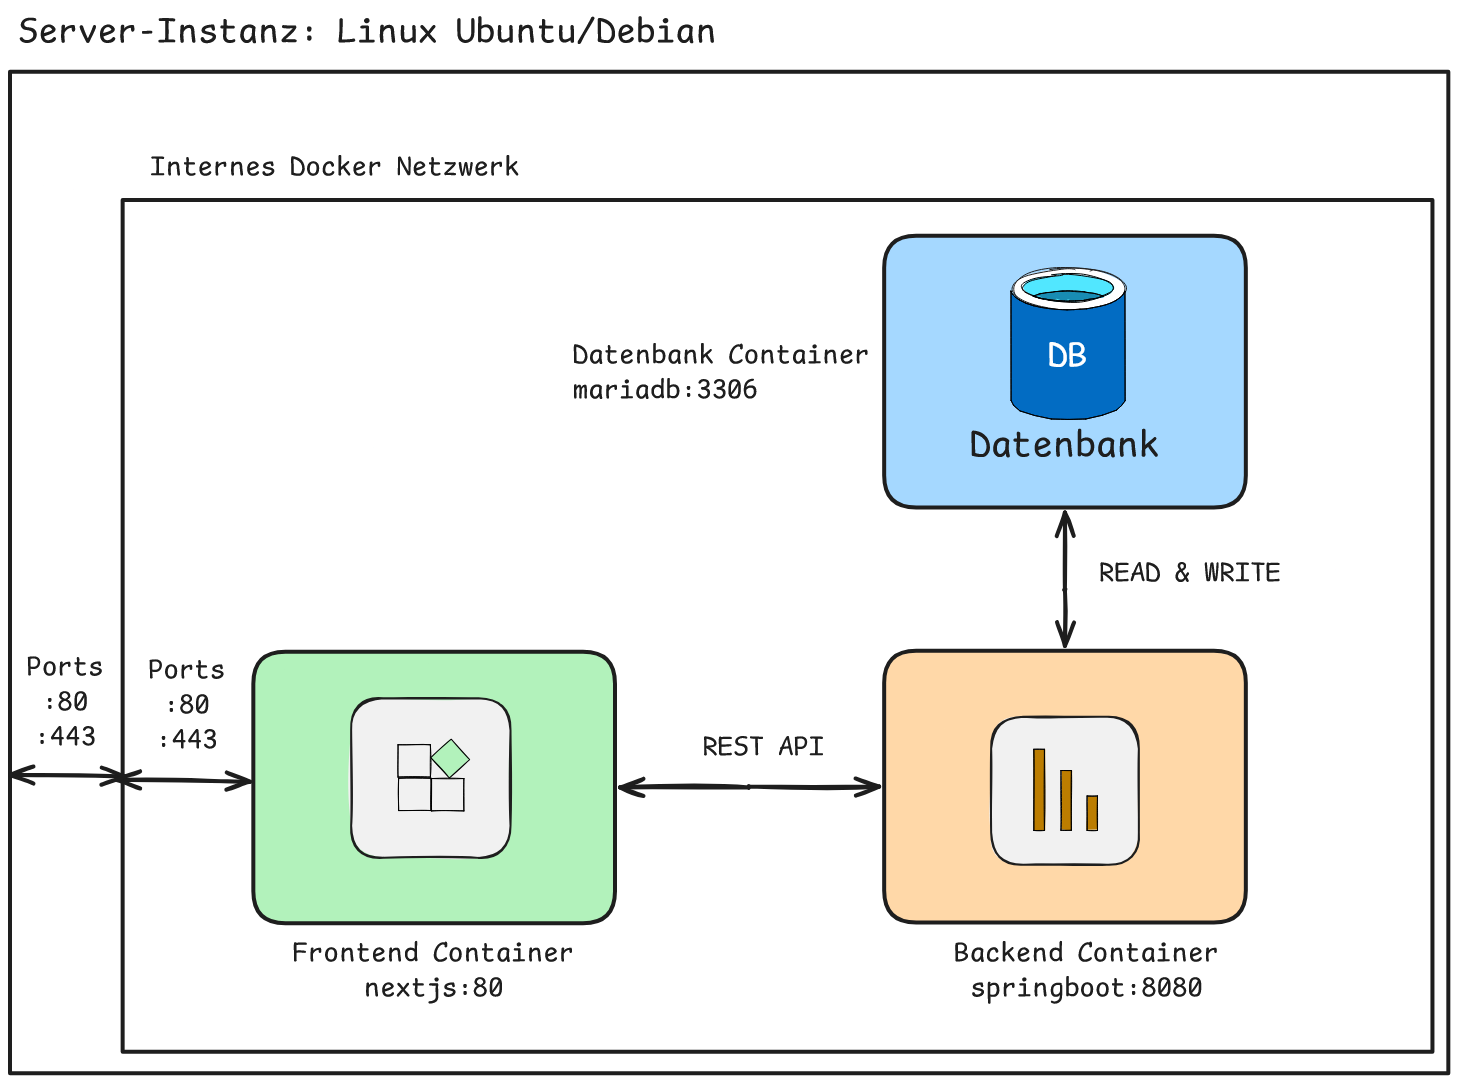
\includegraphics[width=0.9\textwidth]{images/architectural-design.png}
	\caption{Grafische Darstellung des Architekturdesigns. Es gibt hierbei genau 3 Komponenten, welche alle in einem internen Docker Netzwerk untergebracht sind. Darunter fallen das Frontend, das Backend und die Datenbank.}
    \label{koncept-archdesign-backend}
\end{figure}

Wie in Abbildung \ref{koncept-archdesign-backend} dargestellt, wird es drei Hauptkomponenten geben:

\begin{itemize}
	\item Das Frontend: Verantwortlich für die grafische Darstellung der Website und die Entgegennahme von Benutzerdaten.
	\item Das Backend: Verantwortlich für die Verarbeitung der vom Frontend empfangenen Daten und Kommunikation mit der Datenbank.
	\item Die Datenbank: Verantwortlich für die Speicherung aller Daten.
\end{itemize}

Die Applikation wird mit der Container-Technologie Docker \cite{website-docker} ausgeliefert, um den Build-Prozess zu vereinfachen.

\subsection{API-Design und Endpunkte}

Die API-Schnittstelle des Projekts wird mittels \textbf{REST} bereitgestellt, um eine effiziente Kommunikation zwischen Frontend und Backend zu gewährleisten. \textbf{Spring Boot} bietet dabei native Unterstützung für RESTful Web Services \cite{website-spring_rest}.

Folgende Endpunkte sind vorgesehen:
\begin{itemize}
	\item \textbf{POST /api/v1/forms}: Übermittlung eines Formulars vom Frontend an das Backend.
	\item 	\textbf{GET /api/v1/forms}: Anzeige aller gespeicherten Formulare.
	\item \textbf{GET /api/v1/forms/{id}}: Anzeige eines bestimmten Formulars.
	\item \textbf{PUT /api/v1/forms/{id}}: Aktualisierung eines bestehenden Formulars.
	\item \textbf{DELETE /api/v1/forms/{id}}: Löschen eines spezifischen Formulars.
\end{itemize}

Zur Sicherstellung der Datenqualität wird eine \textbf{Datenvalidierung} über die in Spring Boot integrierten Validierungs-Pakete vorgenommen. \textbf{Spring Security}\cite{website-spring_security} wird eingesetzt, um Authentifizierungs- und Autorisierungsfunktionen zu gewährleisten und den Zugriff auf die API-Endpunkte abzusichern.


\subsection{Workflow und Datenfluss}

Um sich jetzt ein konkretes Bild der Funktionalität der Applikation machen zu können, wird hier eine Beispielanfrage analysiert. 

Diese Anfrage soll sicherstellen, dass das Backend die Formulardaten vom Frontend korrekt verarbeitet und speichert.

\newpage

\subsection{Beispielanfrage des Frontends}

Es wurde bereits eine konkrete Datenstruktur entworfen, um diesen Prozess zu optimieren.

Der folgende Text, der im \gls{json}-Format ist, wird vom Frontend an das Backend an \textbf{POST /api/v1/forms} gesendet: \cite{website-git-backend-repo}

\begin{lstlisting}[language=Java, caption={Beispiel-Anfrage an das Backend.}]
...
"accommodation": 1,
"apartmentCountry": "ITALY",
"mainPerson": {
	"mainTraveler": true,
	"firstName": "Mario",
	"lastName": "Rossi",
	"gender": "MALE",
	"birthDate": "1985-04-12",
	"travelDocument": {
		"passportNr": "X12345678",
		"country": "ITALY",
		"issueDate": "2010-05-01",
		"issuing_authority": "Ministero dell'Interno"
...
\end{lstlisting}
		
		\subsection{Abarbeitung der Abfrage}
		
		\begin{figure}
			\centering
			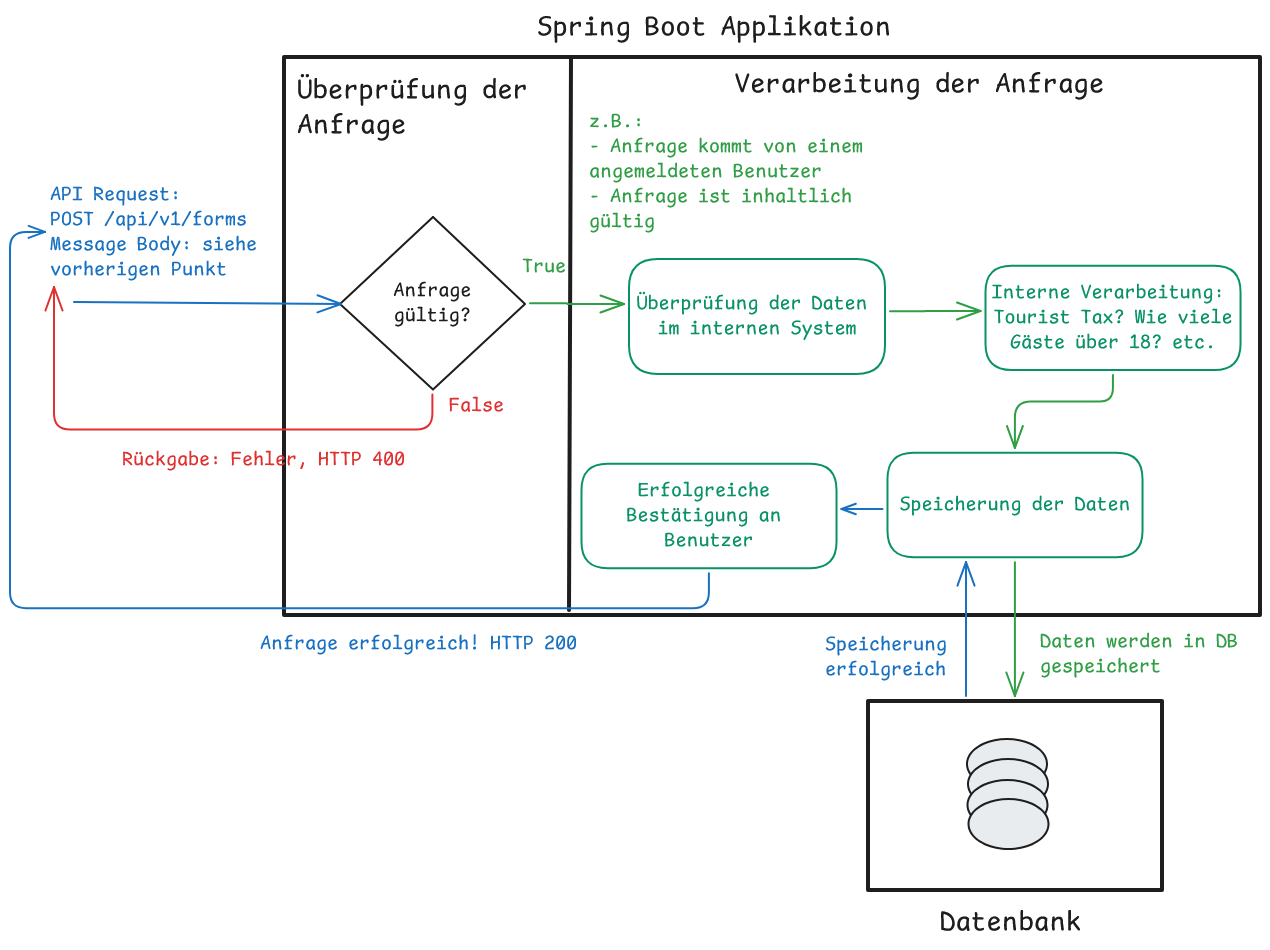
\includegraphics[width=0.9\textwidth]{images/Workflow-backend-post-form.png}
			\caption{Grafische Darstellung des Prozesses der Verarbeitung und Speicherung von Formulardaten im Backend.}
            \label{workflow-form-data-process-backend}
		\end{figure}
		
		Wie in Abbildung \ref{workflow-form-data-process-backend} dargestellt, läuft ein Prozess für die Verarbeitung und Speicherung von Formulardaten in etwa folgendermaßen ab:
		
		\begin{enumerate}
			\item Die Anfrage wird an den Endpunkt \textbf{POST /api/v1/forms} gesendet und auch empfangen.
			\item Die Anfrage wird auf ihre Gültigkeit überprüft: entsprechen die darin enthaltenen Daten der erwarteten Datenstruktur? Sind alle Informationen vorhanden? Falls dies nicht der Fall ist, bekommt der Benutzer einen Fehler angezeigt.
			\item Als Nächstes werden die Daten im internen System validiert. Dies bedeutet, dass z.B. überprüft wird, ob die Reisepassnummer des Hauptreisenden gültig ist, oder ob Daten wie Geburtsdaten usw. gültig sind.
			\item Anschließend werden die Daten intern von der Spring Boot Applikation verarbeitet: Die Objekte werden erstellt und Werte wie zum Beispiel, ob eine italienische Touristensteuer anfällt und wie viele Gäste volljährig sind, werden berechnet.
			\item Danach werden die Daten in die Datenbank eingepflegt. Falls dies erfolgreich gelungen ist, bekommt der Benutzer eine Bestätigung angezeigt.
		\end{enumerate}